%\documentclass[a4paper,superscriptaddress,11pt]{quantumarticle}
\documentclass[aps,twocolumn,longbibliography,english,superscriptaddress,prr]{revtex4-1}
%\documentclass[a4paper,superscriptaddress,11pt]{article}
\pdfoutput=1
\usepackage[colorlinks=true,urlcolor=blue,citecolor=blue,linkcolor=blue]{hyperref}
\usepackage[english]{babel}
\usepackage[utf8]{inputenc}
\usepackage[T1]{fontenc}
\usepackage{amssymb}
\usepackage{tabularx}
\usepackage{upquote}
%\usepackage{multicol}
%\usepackage{caption}
%\usepackage[plain]{algorithm}
\usepackage[ruled, vlined]{algorithm2e}
\usepackage{algpseudocode}
\usepackage{rotating}
%\usepackage{cite}
\usepackage{booktabs}
%\usepackage{unicode-math}
%\usepackage{algorithm}% http://ctan.org/pkg/algorithm
%\usepackage{algpseudocode}% http://ctan.org/pkg/algpseudocode
\usepackage{xcolor}% http://ctan.org/pkg/xcolor
\makeatletter
\newsavebox{\@brx}
\newcommand{\llangle}[1][]{\savebox{\@brx}{\(\m@th{#1\langle}\)}%
  \mathopen{\copy\@brx\kern-0.5\wd\@brx\usebox{\@brx}}}
\newcommand{\rrangle}[1][]{\savebox{\@brx}{\(\m@th{#1\rangle}\)}%
  \mathclose{\copy\@brx\kern-0.5\wd\@brx\usebox{\@brx}}}
\makeatother

\usepackage{bbm}
\usepackage{jlcode}
\usepackage{graphicx, subfigure}
\usepackage{amsmath,color,amsthm}
\usepackage{mathrsfs}
\usepackage{float}
\usepackage[normalem]{ulem}
\usepackage{indentfirst}
\usepackage{txfonts}
\usepackage{listings}
\lstset{
    language=Julia,
    basicstyle=\ttfamily\footnotesize,
    numberstyle=\scriptsize,
    % numbers=left,
    backgroundcolor=\color{gray!10},
    frame=single,
    tabsize=2,
    rulecolor=\color{black!30},
    title=\lstname,
    escapeinside={\%(*}{*)},
    breaklines=true,
    breakatwhitespace=true,
    framextopmargin=2pt,
    framexbottommargin=2pt,
    extendedchars=true,
    inputencoding=utf8,
    columns=fullflexible,
}

\usepackage[epsilon, tsrm, altpo]{backnaur}

\tolerance=1
\emergencystretch=\maxdimen
\hyphenpenalty=1000
\hbadness=1000

\makeatletter

%%%%%%%%%%%%%%%%%%%%%%%%%%%%%% User specified LaTeX commands.

%Journal reference.  Comma sets off: name, vol, page, year
\def\journal #1, #2, #3, 1#4#5#6{{\sl #1~}{\bf #2}, #3 (1#4#5#6) }
\def\pr{\journal Phys. Rev., }
\def\prb{\journal Phys. Rev. B, }
\def\prl{\journal Phys. Rev. Lett., }
\def\pl{\journal Phys. Lett., }
%\def\np{\journal Nucl. Phys., }


%%%%%%%%%%%%%%%%%%%%%%%%%%%%%%%%%%%%%%%%%%%%%%%%%%%%%%%%%%%%%%%%%%%%%%%%%%%%%%%%%%%%%%%%%%%%%%%%%%%%%%%%%%%%%%%%%%%%%%%%%%%%%%%%%%%%%%%%%%%%%%%%%%%%%%%%%%%%%%%%%%%%%%%%%%%%%%%%%%%%%%%%%%%%%%%%%%%%%%%%%%%%%%%%%%%%%%%%%%%%%%%%%%%%%%%%%%%%%%%%%%%%%%%%%%%%


%\usepackage{CJK}
%\usepackage[colorlinks, citecolor=blue]{hyperref}
\DeclareMathOperator*{\argmax}{arg\,max}

%%%%%% Shortcut related
\newcommand{\<}{\langle}
\renewcommand{\>}{\rangle}
\newcommand{\out}{{O}}
\newcommand{\inp}{{I}}
\newcommand{\pluseq}{\mathrel{+}=}
\newcommand{\minuseq}{\mathrel{-}=}
\newcommand{\vx}{{\vec x}}
\newcommand{\vg}{{\vec g}}
\newcommand{\vp}{{\vec p}}
\newcommand{\vy}{{\vec y}}
\newcommand{\vvalue}{{\texttt{value}}}
\newcommand{\grad}{{\texttt{grad}}}
\newcommand{\garbage}{{\texttt{garbage}}}
%%%%%% Convention related
\newcommand{\SWAP}{{\rm SWAP}}
\newcommand{\CNOT}{{\rm CNOT}}
\newcommand{\X}{{\rm X}}
\renewcommand{\H}{{\rm H}}
\newcommand{\Rx}{{\rm Rx}}
\renewcommand{\v}[1]{{\bf #1}}
\newcommand{\dataset}{{\mathcal{D}}}
\newcommand{\wfunc}{{\psi}}
\newcommand{\SU}{{\rm SU}}
\newcommand{\UU}{{\rm U}}
\newcommand{\thetav}{{\boldsymbol{\theta}}}
\newcommand{\gammav}{{\boldsymbol{\gamma}}}
\newcommand{\thetai}{{\theta^\alpha_l}}
\newcommand{\Expect}{{\mathbb{E}}}
\newcommand{\Tr}{{\rm Tr}}
\newcommand{\etc}{{\it etc~}}
\newcommand{\etal}{{\it etal~}}
\newcommand{\xset}{\mathbf{X}}
\newcommand{\fl}{\texttt{fl}}
\newcommand{\pdata}{\mathbf{\pi}}
\newcommand{\q}{\mathbf{q}}
\newcommand{\epdata}{\mathbf{\hat{\pi}}}
\newcommand{\gammaset}{\boldsymbol{\Gamma}}
\newcommand{\ei}{{\mathbf{e}_l^\alpha}}
\newcommand{\vtheta}{{\boldsymbol{\theta}}}
\newcommand{\sigmag}{{\nu}}
\newcommand{\sigmai}[2]{{\sigma^{#2}_{#1}}}
\newcommand{\qi}[1]{{q^{\alpha_{#1}}_{#1}}}
\newcommand{\BAS}{Bars-and-Stripes}
\newcommand{\circled}[1]{\raisebox{.5pt}{\textcircled{\raisebox{-.9pt} {#1}}}}

\newcommand{\qexpect}[1]{{\left\langle #1\right\rangle}}
\newcommand{\expect}[2]{{\mathop{\mathbb{E}}\limits_{\substack{#2}}\left[#1\right]}}
\newcommand{\var}[2]{{\mathop{\mathrm{Var}}\limits_{\substack{#2}}\left(#1\right)}}
\newcommand{\pshift}[1]{{p_{\thetav+#1}}}
\newcommand{\upcite}[1]{\textsuperscript{\cite{#1}}}
\newcommand{\Eq}[1]{Eq.~(\ref{#1})}
\newcommand{\Fig}[1]{Fig.~\ref{#1}}
\newcommand{\Tbl}[1]{Table~\ref{#1}}
\newcommand{\Sec}[1]{Sec.~\ref{#1}}
\newcommand{\App}[1]{Appendix \ref{#1}}
\newcommand{\bra}[1]{\mbox{$\left\langle #1 \right|$}}
\newcommand{\ket}[1]{\mbox{$\left| #1 \right\rangle$}}
\newcommand{\braket}[2]{\mbox{$\left\langle #1 | #2 \right\rangle$}}
\newcommand{\tr}[1]{\mathrm{tr}\mbox{$\left[ #1\right]$}}

\newcommand{\ra}[1]{\renewcommand{\arraystretch}{#1}}

%%%%%% Comment related
\newcommand{\red}[1]{[{\bf  \color{red}{LW: #1}}]}
\newcommand{\xred}[1]{[{\bf  \color{red}{\sout{LW: #1}}}]}
\newcommand{\blue}[1]{[{\bf  \color{blue}{JG: #1}}]}
\newcommand{\xblue}[1]{[{\bf  \color{blue}{\sout{JG: #1}}}]}
\newcommand{\material}[1]{\iffalse[{\bf  \color{cyan}{Material: #1}}]\fi}

\newtheorem{theorem}{\textit{Theorem}}
\theoremstyle{definition}\newtheorem{definition}{\textit{Definition}}

\makeatother

\begin{document}
\title{Instruction level automatic differentiation on a reversible Turing machine}

%\author{Jin-Guo Liu\thanks{cacate0129@iphy.ac.cn}\\
%Institute of Physics, Chinese Academy of Sciences,\\Beijing 100190, China\\
%\And
%Hong-Xuan Zhao-Wang\\
%Department of Computer Science, University of Tsukuba
%}
%\author{Lei Wang}
%\email{wanglei@iphy.ac.cn}
%\affiliation{Institute of Physics, Chinese Academy of Sciences, Beijing 100190, China}
%\affiliation{CAS Center for Excellence in Topological Quantum Computation, University of Chinese Academy of Sciences, Beijing 100190, China}
%\affiliation{Songshan Lake Materials Laboratory, Dongguan, Guangdong 523808, China}

\author{Jin-Guo Liu}
\email{cacate0129@iphy.ac.cn}
\affiliation{Institute of Physics, Chinese Academy of Sciences, Beijing 100190, China}

\author{Taine Zhao}
\affiliation{Department of Computer Science, University of Tsukuba}

\begin{abstract}
    This paper considers the instruction level adjoint mode differential programming, i.e. knowing only the backward rules of basic instructions like +, -, * and /, obtain the gradient of parameters in an arbituary differentiable program with proper performance. In this paper, we review briefly why instruction level automatic differentiation is hard for current machine learning frameworks and propose an implementation of reversible Turing machine as a solution. We show how reversible programming can differentiate a general program to an arbituary order automatically by viewing basic instructions as the computational graph.
\end{abstract}


\maketitle

%\begin{multicols}{2}
\section{Introduction}\label{sec:intro}
    \blue{TODOs: quantum example?}
    There are two modes of automatic differentiation (AD)~\cite{Hascoet2013}, the tangent mode~\cite{Revels2016} and the adjoint mode.
    Consider a multi-in multi-out function $\vy = f(\vx)$, the tangent mode computes one column of its Jacobian $\frac{\partial \vy}{\partial x_i}$ efficiently, where $x_i$ is one of the input variables.
Whereas the adjoint mode computes one row of Jacobian $\frac{\partial y_i}{\partial \vec{x}}$ efficiently.
Most popular automatic differentiation package implements the adjoint mode AD. Because the adjoint mode is computational more efficient in variational applications, where the loss as output is always a scalar.
However, implementing adjoint mode AD is harder than implementing the tangent mode AD. It requires a program's intermediate state for back propagation, including
\begin{enumerate}
    \item the computation graph,
    \item and input variables of nodes in computation graph.
\end{enumerate}
    A computational graph is a directed acyclic graph (DAG) that records the relation between data (edges) and functions (nodes).
In Pytorch~\cite{Paszke2017} and Flux~\cite{Innes2018}, every variable has a tracker field that stores its parent information, i.e. the input data and function that generate this variable. TensorFlow~\cite{Tensorflow2015} implements a static computational graph as a description of the program before actual computation happens.
    Source to source automatic differentiation package Zygote~\cite{Innes2018, Innes2019} use a intermediate representation of a program the static single assignment (SSA) form as the computation graph in order to propagate a native julia code. To cache the intermediate state, it uses a global storage.

    Several limitations are observed in these AD implementions due to the recording and caching. First of all, these package requires a lot primitive functions with programmer defined backward rules. This is not nessesary given the fact that, at the lowest level, these primitive functions are compiled to a finite set of instructions including `+', `-', `*', `/' and conditional jump statements. By defining backward rules for these basic instructions, AD should just works. These machine learning packages can not use instructions as the computational graph for practical reasons. The cost of memorizing the computational graph and caching intermediate states is huge. It can decrease the performance for more than two orders when a program contains loops (as we will show latter).
    Even more, the memory consumption for caching intermediate results increases linearly as time. In many deep learning models like recurrent neural network~\cite{Lipton2015} and residual neural networks~\cite{He2016}, the depth can reach several thousand, the memory wall~\cite{memorywall} can be big problem.
    Secondly, inplace functions are not handled properly in the diagram of computation graph. Even in source to source AD engine Zygote, it is not trivil to handle inplace functions. Most functions in BLAS and LAPACK are implemented as inplace functions. The lack of automatic differentiation support to inplace functions make the memory wall problem even more sevire. It is also harmful to code reusing since all packages using BLAS functions should define their own backward rules for their non-inplace wrappers.
    Thridly, obtaining higher order gradients are not efficient in these packages. For example, in most machine learning packages, people back propagate the whole program of obtaining first order gradient to obtain the second order gradients. The repeated use of back propagation cause exponential overhead with respect to the order of gradients. A better approach to obtain higher order gradients is through Taylor propagation like in JAX~\cite{Bettencourt2019}. However Taylor propagation requires writing rules for all primitives. Besides the exponential overhead, the sorce to source AD engine Zygote suffers from the significant overhead of just in time compiling in Julia language~\cite{Bezanson2017}.

% where the manually derived backwards rule still faces the degenerate spectrum problem (gradients explodes), instruction level AD will return reasonable gradients. With instruction level AD, people don't worry about inplace functions, which may be a huge problem in traditional approaches. We can back propagate over a quantum simulator, where all instructions are reversible two level unitaries (i.e. Jacobian rotation).

%We don't need extra effort to learn meta parameters.~\cite{} Neural ODE is much easier to design~\cite{Chen2018}.

Our solution to these issues is making a program time reversible. Making use of reversibility has been used in machine learning as a promising approach to save memory. People use information buffer~\cite{Maclaurin2015} and reversible activation functions to reduce the memory allocations in recurrent neural network~\cite{MacKay2018} and residual neural networks~\cite{Behrmann2018}. However, the use of reversiblity in these cases are not general purposed.

Hence we develop a embeded domain specific language (eDSL) in Julia language that implements reversible Turing machine.~\cite{Perumalla2013,Frank2017}.
The gradient of any program writting in this eDSL can be obtained in comparable time with the forward computation. The implementation of AD is similar to \texttt{ForwardDiff}~\cite{Revels2016} but runs backward.
    There has been some prototypes of reversible languages like Janus~\cite{Lutz1986}, R (not the popular one)~\cite{Frank1997}, Erlang~\cite{Lanese2018} and object oriented ROOPL~\cite{Haulund2017}. These languages have reversible control flow that allowing user to input an additional postcondition in control flows to help programs run backward.
    In the past, the main motivation of making a program time reversible is to support reversible devices. Reversible devices do not have a lower bound of energy consumption by Landauer principle~\cite{Landauer1961}. However CMOS devices still has two orders~\cite{Frank2017} space to optimize regarding this lower bound.
    The main contribtion of our work is breaking the information barrier between machine learning community and reversible programming community, providing yet another strong motivation to develop a reversible programming.
    Our eDSL borrows the design of reversible control flow in the Janus, meanwhile provides multiple dispatch based abstraction. With these additional features, the AD engine differentiating a general program could be implemented in less than 100 lines.
Our eDSL generates native julia code, and is completely compatible with Julia language.
Potensial applications includes
\begin{enumerate}
    \item generate AD rules for primitive functions like \texttt{exp},
    \item control problem in robotics~\cite{Giftthaler2017} where tensor is not the dominating data type,
    \item differentiating over reversible integrators~\cite{Laikov2018} without intermediate state caching,
    \item Stablize linear algebras functions backward rules. Current backward rules for singular value decomposition (SVD) and eigenvalue decomposition (ED)~\cite{Seeger2017,Wan2019,Hubig2019} are vulnarable to spectrum degeneracy. The development of backward rules for these linear algebra functions can greatly change the researches in physics~\cite{Xie2020,Liao2019}.

\end{enumerate}

    In this paper, we first introduce the design of this eDSL in \Sec{sec:lang}. On this eDSL, we show how to back propagation Jacobians and Hessians.
    Then we propose a training strategy in \Sec{sec:train} that uses reversibility, rather than gradients.
    In \Sec{sec:example}, we show several examples.
    In \Sec{sec:discussion}, we discuss on several important issues, how time space tradeoff works, reversible instructions and hardwares and finally an outlook to some open problems to be solved.

    \section{Language design}\label{sec:lang}
In a mordern programming language, functions are pushed to a global stack for scheduling. The memory layout of a function is consisted of input arguments, a function frame with informations like return address and saved memory segments, local variables and working stack. After each call, the function clears the input arguments, function frame, local variables and working stack, only stores the return value.
    In the reversible programming style, this kind of design pattern is nolonger the best practise, input variables can not be easily discarded after a function call, since discarding information may ruin reversibility. Hence, a reversible instruction or a function call in our eDSL NiLang changes inputs "inplace".
NiLang is a reversible eDSL in Julia that simulates reversible Turing machine. The grammar is shown in \App{app:grammar}.
Its main feature is contained in a single macro \texttt{@i}. It interprets a function to a finite set of ``instructions'' written in julia language. At the same time, it generates the inverse of this function. The target instructions are closed under the inverse operation ``$\sim$'', hence all functions defined in NiLang are also closed under ``$\sim$'' operations. To design such a eDSL, we first introduce a reversible IR that used in NiLang.

\subsection{Reversible IR}

\begin{figure}
    \centerline{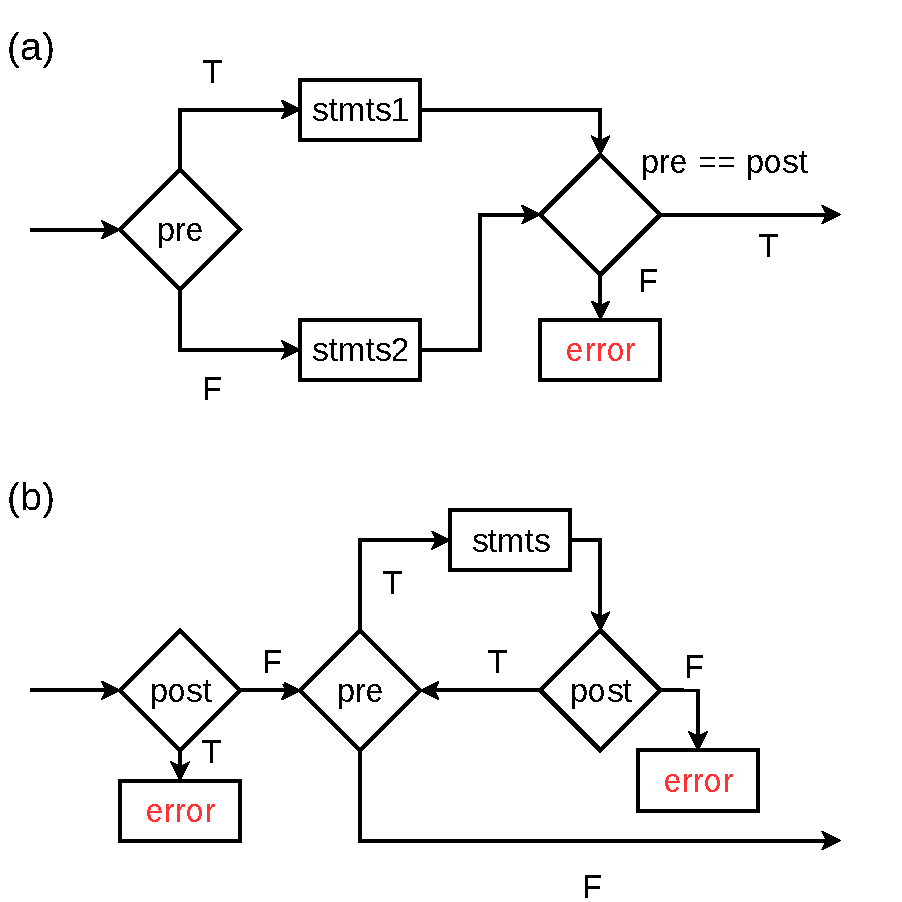
\includegraphics[width=0.7\columnwidth,trim={0 0cm 0 0cm},clip]{images/controlflow.pdf}}
    \caption{Flow chart for reversible (a) \texttt{if} statement and (b) \texttt{while} statement. ``stmts'', ``stmts1'' and ``stmts2'' are statements, statements in true branch and statements in false branch respectively. ``pre'' and ``post'' are precondition and postconditions respectively. ``error'' refers to \texttt{InvertibilityError}.}\label{fig:controlflow}
\end{figure}

\begin{table}[h!]\centering
\begin{minipage}{\columnwidth}
\ra{1.3}
    \scalebox{1.0}{
        \begin{tabularx}{\textwidth}{X X}\toprule
            \textbf{statement} & \textbf{inverse}\\
            \hline
            \texttt{<f>(<args>...)} & \texttt{($\sim$<f>)(<args>...)}\\
            \hline
            \texttt{<y!> += <f>(<args>...)} & \texttt{<y!> -= <f>(<args>...)}\\
            \hline
            \texttt{<y!> .+= <f>.(<args>...)} & \texttt{<y!> .-= <f>.(<args>...)}\\
            \hline
            \texttt{<y!> $\veebar$= <f>(<args>...)} & \texttt{<y!> $\veebar$= <f>(<args>...)}\\
            \hline
            \texttt{<y!> .$\veebar$= <f>(<args>...)} & \texttt{<y!> .$\veebar$= <f>(<args>...)}\\
            \hline
            \texttt{@anc <a> = <expr>} & \texttt{@deanc <a> = <expr>}\\
            \hline
            \texttt{begin\newline $_\quad$<stmts>\newline end} & \texttt{begin\newline $_\quad$ $\sim$(<stmts>)\newline end}\\
            \hline
            \texttt{if (<pre>, <post>)\linebreak $_\quad$<stmts1>\newline else\newline $_\quad$<stmts2>\newline end} & \texttt{if (<post>, <pre>)\newline $_\quad$$\sim$(<stmts>)\newline else\newline $_\quad$ $\sim$(<stmts>)\newline end}\\
            \hline
            \texttt{while (<pre>, <post>)\newline $_\quad$<stmts> \newline end} & \texttt{while (<post>, <pre>)\newline $_\quad$ $\sim$(<stmts>)\newline end}\\
            \hline
            \texttt{for <i>=<m>:<s>:<n>\newline $_\quad$<stmts>\newline end} & \texttt{for <i>=<m>:-<s>:<n>\newline $_\quad$ $\sim$(<stmts>)\newline end}\\
            \hline
            \texttt{@safe <expr>} & \texttt{@safe <expr>}\\
            \bottomrule
        \end{tabularx}
    }
    \caption{A collection of reversible statements.}\label{tbl:revstatements}
\end{minipage}
\end{table}

In NiLang's IR, a statement can be an instruction, a function call, a controlflow, a macrocall or the inverse statement $\sim$.
With the reversible IR, the inverse statement can be defined easily as shown in  in \Tbl{tbl:revstatements}.
An instruction \texttt{y! += f(args...)} is interpreted as a julia function call \texttt{PlusEq(f)(y!, args...)} or \texttt{$\oplus$(f)(y!, args...)} as a shorthand.
Here, the ``!'' after a variable is used as a convension to indicate that a variable is changed after the call of an instruction or function.
The detailed specification of instructions is listed in \App{app:instr}. The function call is same as the host language, except every function \texttt{f} has a \texttt{$\sim$f} that binded to an object of type \texttt{Inv\{typeof(f)\}}. \texttt{$\sim$f} invokes the compiled inverse functions of \texttt{f}.

The reversible control flow is different from the irreversible one that a condition expression in a \texttt{if} or a \texttt{while} statements is a two-element tuple that consist of a precondition and a postcondition. This design allows user putting additional postcondition in control flows to help reverse the program.
A postcondition is a boolean expression that being evaluated after the body expressions being executed.
For the \texttt{if} statement as shown in \Fig{fig:controlflow} (a), the program checks the consistency of precondition and postcondition to make sure they are same. In the reverse pass, the program enters the branch specified by the postcondition.
For the \texttt{while} statement as shown in \Fig{fig:controlflow} (b), before entering, the program check the postcondition to make sure it is false.
After each iteration, the program asserts the postcondition to be true. The inverse function exchanges the precondition and postcondition.
The reverse of \texttt{for} statement is straightforward.
The program first stores the loop informations, start, step and stop, after the execusion of the loop, the program checks the values of these variables are not changed. The reverse program exchanges start and stop and inverse the sign of step.

    There is no assign statements in a reversible language, a reversible replacement is the macro \texttt{@anc}. \texttt{@anc a = <expr>} binds variable \texttt{a} to an initial value specified by \texttt{<expr>}. Its inverse \texttt{@deanc a = <expr>} deallocates the variable \texttt{a}. Before deallocating the variable, the program checks that the value of variable is same as the value of \texttt{<expr>} (or restored), otherwise throws an \texttt{InvertibilityError}. \texttt{@anc} and \texttt{@deanc} must appear in pairs inside a function call, a while statement or a for statement.
    \texttt{@deanc} will be added automatically. Similar designs in Janus and R are \texttt{local/delocal} statement and \texttt{let} statement. The additional check underlines the difference between the irreversible assign statement and reversible ancilla statement.
The \texttt{@safe} macro can be followed by an arbituary statement, it allows user to use external statements that does not break reversibility.
For example, one can use \texttt{@safe @show var} for debugging.

\subsection{Compiling stages}
The interprecation of a reversible function consists three stages.
The first stage preprocess human inputs to a reversible IR, 
The second stage generates the reversed IR according to table \Tbl{tbl:revstatements}.
The third stage is translating this reversible IR to native Julia code.
The following example shows how to compile an \texttt{if} statement

\begin{minipage}{.44\textwidth}
\begin{lstlisting}
julia> using NiLangCore, MacroTools

julia> ex0 = :(if (x > 3, ~)
            grad(arr[3].value) += x * y
        end);
        
julia> ex0 |> prettify
:(if (x > 3, ~)
      grad((arr[3]).value) += x * y
  end)

julia> ex1 = NiLangCore.precom_ex(ex0,
        NiLangCore.PreInfo());
        
julia> ex1 |> prettify  # after stage 1
:(if (x > 3, x > 3)
      grad((arr[3]).value) += x * y
  else
  end)

julia> ex2 = NiLangCore.dual_ex(ex1);

julia> ex2 |> prettify  # after stage 2
:(if (x > 3, x > 3)
      grad((arr[3]).value) -= x * y
  else
  end)

julia> ex3 = NiLangCore.interpret_ex(ex2);

julia> ex3 |> prettify  # after stage 3
quote
    wren = x > 3
    if wren
        @instr grad((arr[3]).value) -= x * y
    else
    end
    @invcheck x > 3 wren
end
\end{lstlisting}
\end{minipage}

In the first stage, the preprocessor expands the symbol \texttt{$\sim$} in postcondition field of \texttt{if} statement to the precondition as shown above. Besides, it adds missing \texttt{@deanc} to ensure \texttt{@anc} and \texttt{@deanc} statements appear in pairs and  expands \texttt{@routine} macro.
\texttt{@routine r Stmt} records a statement to symbol \texttt{r}. When \texttt{$\sim$@routine r} is called, the inverse statement is inserted to that position for uncomputing.
In the last stage, the compiler adds \texttt{@instr} before each instruction and function call statement,
The macro \texttt{@instr} assign the output of a function to the argument list of a function. We will explain this macro in detail in next subsection.
It also adds statements to check the consistency between preconditions and postconditions to ensure reversibility,
Finally, at the end of a function body, it attaches a return statement that uses input variables as the output.
Now the function is ready to execute on the host language.

\subsection{Types and Dataviews}
The constructor of a type is also a reversible function.
The inverse function is a ``destructor'', which does not deallocate memory directly but unpacks data.

\begin{minipage}{.44\textwidth}
\begin{lstlisting}
using NiLangCore, Test

struct DVar{T}
    x::T
    g::T
end

@iconstruct function DVar(xx, gg=zero(xx))
    gg += identity(xx)
end

@test (~DVar)(DVar(0.5)) == 0.5
\end{lstlisting}
\end{minipage}

The \texttt{@iconstruct} generates a reversible constructor with single parameters \texttt{xx} as input. The statement \texttt{gg = zero(xx)} initializes a new memory to be used. The body of function is a reversible program that modifies \texttt{xx} and \texttt{gg}. Finally call the default constructor \texttt{DVar(xx, gg)}. It is easy to find the inverse procedure that transform a \texttt{DVar{T}} instance to a \texttt{T} instance. With the flexibility to operate types, it is not nessesary to use global stacks in our eDSL.

Before introducing dataviews, let's first consider the following line that appear in the last subsection

\begin{minipage}{.44\textwidth}
\begin{lstlisting}
grad(arr[3].value) += x * y
\end{lstlisting}
\end{minipage}

In Julia, this statement will raise a syntax error, since a function call can not be assigned.
Meanwhile \texttt{arr[3]} might be a immutable type.
In our eDSL, we wish it works because every memory cell should be modifiable ``inplace''.

As we have mensioned, \texttt{grad(arr[3].value) += x * y} is translated to \texttt{@instr grad(arr[3].value) += x * y} at the thrid stage.
To execute the instruction, \texttt{@instr} translate the statement to

\begin{minipage}{.44\textwidth}
    \begin{lstlisting}[numberstyle=\scriptsize\color{codegray},numbers=left,numbersep=8pt]
res = PlusEq(*)(grad(arr[3].value), x, y)
arr[3] = chfield(arr[1], Val(:value), 
    chfield(arr[3].value, grad, res[1]))
x = res[2]
y = res[3]
\end{lstlisting}
\end{minipage}

\texttt{PlusEq(*)(grad(arr[3].value), x, y)} computes the output, which is a tuple of length $3$.
\texttt{chfield} is used to a dataview.
The second and third arguments can be assigned back directly.
A dataview of a data can be data itself, a field of its view, an array element of its view, or a bijective mapping of its view.
If the default constructor of a type is not overwritten by user, NiLang can modify a field of that type automatically.
For a bijective mapping of a field, user need to specify the behavior of a dataview by overloading \texttt{chfield} function.

\section{Taylor propagation on a reversible Turing machine}\label{sec:bp}
Taylor propagation is exponentially (as the order) more efficient in obtaining higher order gradients than differentiating lower order gradients recursively.
The later requires traversing the computational graph repeatedly.
In JAX, in order to support Taylor propagation, the propagation rules for part of primitives manually defined.
The exhaused support requires much more effort than the first order gradient propagation.
Instruction level automatic differentiation is more flexible in obtaining higher order gradients like Hessian.

\subsection{First order gradient}\label{sec:jacobian}
Given a node $\vec y = f(\vec x)$ in a computational graph, we can propagate the Jacobians in tangent mode like
\begin{align}
    J^\out_{x_i} = J^\out_{y_j} J^{y_j}_{x_i}
\end{align}
and the adjoint mode
\begin{align}
    J^{y_j}_\inp = J^{y_j}_{x_i} J_\inp^{x_i}
\end{align}

Here, $\inp$ is the inputs and $\out$ is the outputs.
Einstein's notation is used so that duplicated indices are summed over.
Tagent mode instruction level automatic differentiation can be implemented easily in a irreversible language with dual numbers,
here we focus on the adjoint mode.
The backward rule can be described in tensor network~\cite{} language as shown in \Fig{fig:ad}.
\begin{figure}
    \centerline{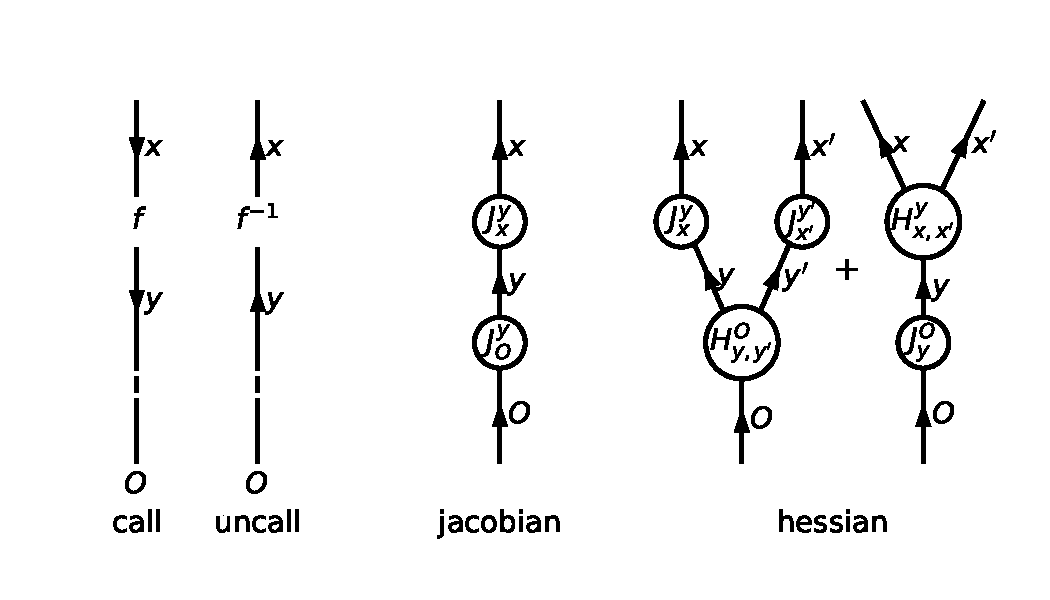
\includegraphics[width=0.9\columnwidth,trim={0.5cm 1cm 0 1cm},clip]{images/ad.pdf}}
    \caption{Adjoint rules for Jacobians and Hessians in tensor network language.}\label{fig:ad}
\end{figure}

In reversible programming, we have the following implementation
\begin{algorithm}[H]
    \KeResult{\grad.($\vx_g$)}
    let \texttt{iloss} be the index of loss variable
    $\vy = f(\vx)$\\
    $\vy_g$ = \texttt{GVar}.($\vy$)\\
    $\vx_g = f^{-1}(\vy_g)$\\
    \grad($\vy_g$[\texttt{iloss}]) += 1.0
    \caption{Reversible programming AD}
\end{algorithm}

Here, ``.'' is the broadcast operations in Julia. \texttt{GVar} is a ``reversible type''. \texttt{GVar(x)} attaches a zero gradient field to a variable, which is similar to the dual number in tangent mode automatic differentiation. The gradient can be accessed by \texttt{grad} function. Its inverse \texttt{$\sim$GVar} deallocates the gradient field safely and returns its value field. Here, "safely" means it will check the gradient field to make sure it is in $0$ state.
When a \texttt{instruct} meets a \texttt{GVar}, besides computing its value field $\vvalue(\vx) = f^{-1}(\vvalue(\vy))$, it also updates the gradient field $\grad(\vx) = J^{\vx}_{\vy} \grad(\vy)$. Since $f^{-1}$ is bijective, $J^\vy_\vx$ can be easily obtained by inspecting its inverse function $f$.
The final output is stored in the gradient field, when then gradient is not used anymore, the faithful reversible programming style to compute gradients would be uncomputing the whole process to obtain gradient, which increases the hyrachy by 1. Whenever the hyrachy increase by 1, the computational overhead doubles comparing with its irreversible counter part.

Due to the multiple dispatch and just in time compiling, most runtime overhead can be removed. Let's consider a simple example that acccumulate $1.0$ to a target variable $x$ for $n$ times

\begin{minipage}{.44\textwidth}
\begin{lstlisting}
@i function prog(x, one, n::Int)
    for i=1:n
        x += identity(one)
    end
end
\end{lstlisting}
\end{minipage}

\begin{figure}
    \centerline{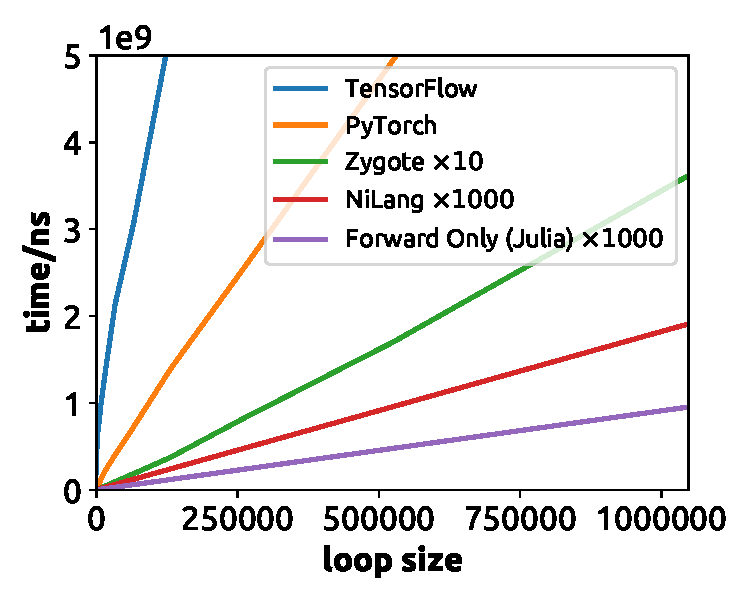
\includegraphics[width=0.9\columnwidth,trim={0 0cm 0 0},clip]{images/fig3.pdf}}
    \caption{The time for obtaining gradient as function of loop size. $\times n$ in lengend represents a rescaling of time.}\label{fig:benchmark}
\end{figure}
From the benchmark result shown in \Fig{fig:benchmark}.
One can see that the NiLang implementation is unreasonablely fast, even faster than two times the forward pass written in Julia. The code for benchmark is open for review in our paper github repository~\cite{nilangpaper}.
This benchmark does show the actual performance in real applications.
In real application, the reversible program can have memory or computing time overhead. We will discuss the details of time and space tradeoff in \Sec{sec:timespace}.

\subsection{Second order gradient}
The second order gradient can also be back propagated
\begin{align}
    \begin{split}
        &H^f_{y_L,y_L'} = 0\\
        &H^f_{y_{i-1},y_{i-1}'} = J^{y_i}_{y_{i-1}} H^f_{y_i, y_i'} J^{y_i'}_{y_{i-1}'} + J^f_{y_i} H^{y_i}_{y_{i-1}, y_{i-1}'}
    \end{split}
\end{align}

In tensor network language, it can be represented as in \Fig{fig:ad}.
This approach can be easily extended to higher orders, or taylor propagation.
However, this is not the widely adopted approach to compute higher order gradients.
Althought backpropagating higher order gradients directly is exponentially faster than back propagating the computational graph for computing lower order gradients for computing higher order gradients, one has to extending the backward rules for each primitive rather than reusing existing ones.
Here, we emphasis that with instruction level AD, rewritting backward rules for primitives turns out to be not so difficult.
An example is provided in \Sec{sec:exp}.

\subsection{Gradient on ancilla problem}
Ancilla can also carry gradients during computation, sometimes these gradients can not be uncomputed even if their parents can be uncomputed regoriously. In these case, we simply ``drop'' the gradient field instead of raising an error. In this subsection, we prove doing this is safe, i.e. does not have effect on rest parts of program.

Ancilla is the fixed point of a function, which means 
\begin{align}
    \begin{split}
    &b, y \leftarrow f(x, a)\; \text{, where } b==a\\
    &\frac{\partial b}{\partial x} = 0
    \end{split}
\end{align}

During the computation, the gradient field does not have any effect to the \texttt{value} field of variables. The key question is will the loss of gradient part in ancilla affect the reversibility of the gradient part of argument variables.
The gradient of argument variable is defined as $\frac{\partial L}{\partial x} = \frac{\partial L}{\partial y}\frac{\partial y}{\partial x} + \frac{\partial L}{\partial b}\frac{\partial b}{\partial x}$, where the second term vanish naturally.

\subsection{Implementation}
The automatic differentiation engine is so short that we present the function defintion as follows

\begin{minipage}{.44\textwidth}
\begin{lstlisting}
@i function (g::Grad)(args...; kwargs...)
    @safe @assert count(x -> x isa Loss, args) == 1
    @anc iloss = 0
    @routine getiloss begin
        for i=1:length(args)
            if (tget(args,i) isa Loss, iloss==i)
                iloss += identity(i)
                (~Loss)(tget(args,i))
            end
        end
    end

    g.f(args...; kwargs...)
    GVar.(args)
    grad(tget(args,iloss)) += identity(1.0)
    (~g.f)(args...; kwargs...)

    ~@routine getiloss
end
\end{lstlisting}
\end{minipage}

The program first checks the input parameters and locate the loss variable.
Then \texttt{~Loss} unwraps the loss variable, the location of loss variable is transferred to the ancilla \texttt{iloss} of integer type.

\texttt{GVar}

\begin{minipage}{.44\textwidth}
\begin{lstlisting}
julia> using NiLang, NiLang.AD

julia> x, y = GVar(0.5), GVar(0.6)
(GVar(0.5, 0.0), GVar(0.6, 0.0))

julia> @instr grad(x) += identity(1.0)

julia> @instr x += identity(y)

julia> y
GVar(0.6, -1.0)

julia> @instr grad(x) -= identity(1.0)

julia> @instr (~GVar)(x)

julia> x
1.1
\end{lstlisting}
\end{minipage}

Broadcasting is supported. To avoid possible confusing, tuple indexing is forbidden delebrately, one can use \texttt{tget(tuple, 2)} to get the second element of a tuple.

\section{Learn by consistency}\label{sec:train}
Consider training data consist of input $\vx^*$ and output $\vy^*$.
The goal is to find a set of parameters $\vp_x$ that satisfy $\vy^* = f(\vx^*, \vp_x)$.
In traditional machine learning, we define a loss $\mathcal{L} = {\rm dist}(\vy^*, f(\vx^*, \vp_x))$ and minimize it with gradient $\frac{\partial L}{\partial \vp_x}$. This is viable only when the target function is locally differentiable.

Here we provide an alternative by making use of reversibility.
We construct a reversible program $\vy, \vp_y =  f_r(\vx, \vp_x)$, where $\vp_x$ and $\vp_y$ are ``garbage'' spaces which include parameters.
The algorithm can be summarized as

\begin{algorithm}[H]
    \KwResult{$\vg_x$}
    Initialize $\vx$ to $\vx^*$, garbage space $\vg_x$ to random.\\
    \eIf{$\vg_y$ is \texttt{null}}{
        $\vx, \vg_x = f_r^{-1}(\vy^*)$\\
    }{
        $\vy, \vg_y= f_r(\vx, \vg_x)$\\
        \While{$\vy \not\approx \vy^*$}{
            $\vy = \vy^*$\\
            $\vx, \vg_x = f_r^{-1}(\vy, \vg_y)$.\\
            $\vx = \vx^*$\\
            $\vy, \vg_y= f_r(\vx, \vg_x)$
        }
    }
    \caption{Learn by consistency}\label{algo:train}
\end{algorithm}

Here, $\garbage(\cdot)$ is a function for taking the garbage space.
This algorithm utilizes the self-consistency relation
\begin{equation}\label{eq:selfconsistent}
    \vg_x^* = \garbage(f_r^{-1}(\vy^*, \garbage(f_r(\vx^*, \vg^*_x)))),
\end{equation}

Similar idea of training by consistency is used in self-consistent meanfield theory~\cite{} in physics.
The difficult part of self-consistent training is to find a self-consistency relation, here the reversibility provides a natural self-consistency relation.
Learn by consistency can be used to handle descrete optimization. However, it is not a silver bullet, and should be used with causion.
Let's consider the following example

\begin{minipage}{.44\textwidth}
\begin{lstlisting}[basicstyle=\small\ttfamily,columns=fullflexible]
@i function f1(out!, x, y!)
    y! += identity(x)
    out! -= exp(x)
    out! += exp(y!)
end

@i function f2(out!, x!, y!)
    y! += identity(x!)
    out! -= exp(x!)
    x! -= log(-out!)
    out! += exp(y!)
end

function train(f)
    loss = Float64[]
    y = 1.6
    for i=1:100
        out!, x = 0.0, 0.3
        @instr f(out!, x, y)
        push!(loss, out!)
        out! = 1.0
        @instr (~f)(out!, x, y)
    end
    loss
end
\end{lstlisting}
\end{minipage}

Functions \texttt{f1} and \texttt{f2} computes $f(x, y) = e^{(y+x)} - e^x$ and stores the output in a new memory \texttt{out!}.
The only difference is $f_2$ ``uncompute'' $x$ arithmetically.
The task of training is to find a $y$ that make the output value equal to target value $1$.
After $200$ steps, $f_2$ runs into the fixed point with $x$ equal to $1$ upto machine precision.
However, $f_1$ does not do any training.
The training of $f_2$ fails because this function actually computes $f_1(out!, x, y!) = out! + e^{(y!+x)} - e^x, x, x+y!$, where the training parameter $y$ is completely determined by the garbage space on output side $x$ and $x+y!$. As a result, shifting $out!$ directly is the only approach to satisfy the consistency relation. On the other side, $f_2(out!, x, y!) = out! + e^{(y!+x)} - e^x, \left(x-\log(e^x)\right), x+y!$, parameters $y$ is not completely determined by the garbage space $\left(x-\log(e^x)\right), x+y!$.

\begin{figure}
    \centerline{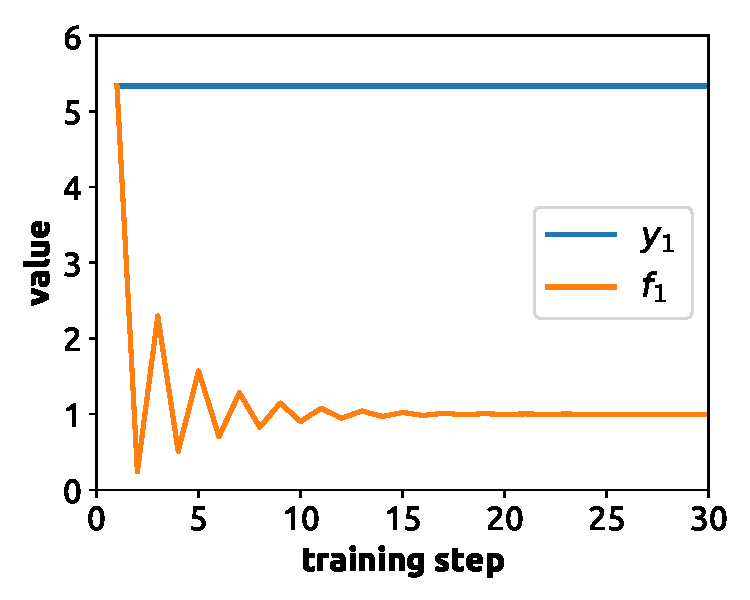
\includegraphics[width=0.9\columnwidth,trim={0 0.3cm 0 0},clip]{images/fig1.pdf}}
    \caption{The value of $x$ as a function of self-consistent training step.}\label{fig:invtrain}
\end{figure}

By viewing $\vx$ and parameters in $\vp_x$ as variables, we can study the trainability from the information perspective.
\begin{theorem}
    Only if the the conditional entropy $S(\vy|\vp_y)$ is nonzero, algorithm \ref{algo:train} is trainable.
\end{theorem}
\begin{proof}
The above discussion reveals a fact that the training can not work when the output $\vp_y$ completely determines $\vp_x$, that is
\begin{align}
    \begin{split}
        S(\vp_x | \vp_y) &= S(\vp_x \cup \vp_y) - S(\vp_y)\\
        &\leq S\left((\vp_x \cup \vx) \cup \vp_y \right) - S(\vp_y),\\
        &\leq S\left((\vp_y \cup \vy) \cup \vp_y\right) - S(\vp_y),\\
    &\leq S(\vy|\vp_y).
    \end{split}
\end{align}
The third line uses the bijectivity $S(\vx \cup \vp_x) = S(\vy \cup \vp_y)$.
\end{proof}
This inequality shows that when the garbage space on the output side satisfies $S(\vy | \vp_y) = 0$, i.e. contains all information to determine the output field, the input parameters are also completely determined by this garbage space.
In the above examples, it corresponds to the case $S\left(e^{(x+y)-e^x} | x \cup x + y\right) = 0$ in $f_1$.
One should remove the redundancy of information by uncomputing to make training by consistency work properly.

\section{Examples}\label{sec:example}

\subsection{Computing Fibonacci Numbers}\label{sec:fib}
An example that everyone likes

\begin{minipage}{.44\textwidth}
\begin{lstlisting}
@i function rfib(out, n::T) where T
    @anc n1 = zero(T)
    @anc n2 = zero(T)
    @routine init begin
        n1 += identity(n)
        n1 -= identity(1.0)
        n2 += identity(n)
        n2 -= identity(2.0)
    end
    if (value(n) <= 2, ~)
        out += identity(1.0)
    else
        rfib(out, n1)
        rfib(out, n2)
    end
    ~@routine init
end
\end{lstlisting}
\end{minipage}

To compute the first Fibonacci number that is greater or equal to 100

\begin{minipage}{.44\textwidth}
\begin{lstlisting}
@i function rfib100(n)
    @safe @assert n == 0
    while (fib(n) < 100, n != 0)
        n += identity(1.0)
    end
end
\end{lstlisting}
\end{minipage}

Here, \texttt{fib} and \texttt{rfib} are defined in \App{sec:fib}.

\subsection{exp function}\label{sec:exp}
An $\exp$ function can be computed using Taylor expansion
\begin{equation}
    {\rm out!} += \sum\limits_n \frac{x^n}{{\rm factorial}(n)}
\end{equation}
This is a recursive algorithm that mimics pebble game.
Define the term for accumulation $s_n \equiv \frac{x^n}{{\rm factorial}(n)}$, the recursion relation is written as $s_n = \frac{x s_{n-1}}{n}$. There is no known constant memory and polynomial time algorihm to pebble game.
Here the case is different. Notice $*=$ and $/=$ are arithmetically reversible to each other, we can uncompute $s_{n-1} = \frac{n s_n}{x}$ to deallocate memory.
By allowing loss of several digit precision of result, implementing the constant memory reversible $\exp$ function is possible

\begin{minipage}{.44\textwidth}
\begin{lstlisting}
using NiLang, NiLang.AD

@i function iexp(out!, x::T; atol::Float64=1e-14)
        where T
    @anc anc1 = zero(T)
    @anc anc2 = zero(T)
    @anc anc3 = zero(T)
    @anc iplus = 0
    @anc expout = zero(T)

    out! += identity(1.0)
    @routine r1 begin
        anc1 += identity(1.0)
        while (value(anc1) > atol, iplus != 0)
            iplus += identity(1)
            anc2 += anc1 * x
            anc3 += anc2 / iplus
            expout += identity(anc3)
            # arithmetic uncompute
            anc1 -= anc2 / x
            anc2 -= anc3 * iplus
            SWAP(anc1, anc3)
        end
    end

    out! += identity(expout)

    ~@routine r1
end
\end{lstlisting}
\end{minipage}

The definition of SWAP instruction can be found in \App{app:instr}.
The two lines bellow the comment ``\texttt{\# arithmetic uncompute}'' "uncomputes" variables \texttt{anc1} and \texttt{anc2}, this uncomputation is only true arithmeticly, but not for floating point number due to the rouding error. As a result, the final output is not exact due to the rounding error. On the other side, the reversibility is not harmed since the inverse call at the last line of function uncomputes all ancilla bits rigorously.
The \texttt{while} statement takes two conditions, the precondition and postconditoin. Precondition \texttt{val(anc1) > atol} indicates when to break the forward pass and post condition \texttt{!isapprox(iplus, 0.0)} indicates when to break the backward pass.

To obtain the gradient, one can wrap the loss with \texttt{Loss} type and feed it into \texttt{iexp\textsinglequote} function

\begin{minipage}{.44\textwidth}
\begin{lstlisting}
julia> out!, x = 0.0, 1.6
(0.0, 1.6)

julia> @instr iexp'(Loss(out!), x)

julia> grad(x)
4.9530324244260555

julia> out!, x = 0.0, 1.6
(0.0, 1.6)

julia> simple_hessian(iexp, (Loss(out!), x))
2×2 Array{Float64,2}:
 0.0  0.0
 0.0  4.95303
\end{lstlisting}
\end{minipage}

\texttt{iexp\textquotesingle} returns an object of type \texttt{Grad\{typeof(exp)\}}, it returns input variables with updated gradient field.
The loss variable is specified by a wrapper \texttt{Loss}, notice we don't distinguish input and output in reversible programming.
The gradient functions are implemented reversibally so that the gradients can be differentiated again to obtain Hessians as shown in \Fig{fig:simplehessian}.

\begin{figure}[h]
    \centerline{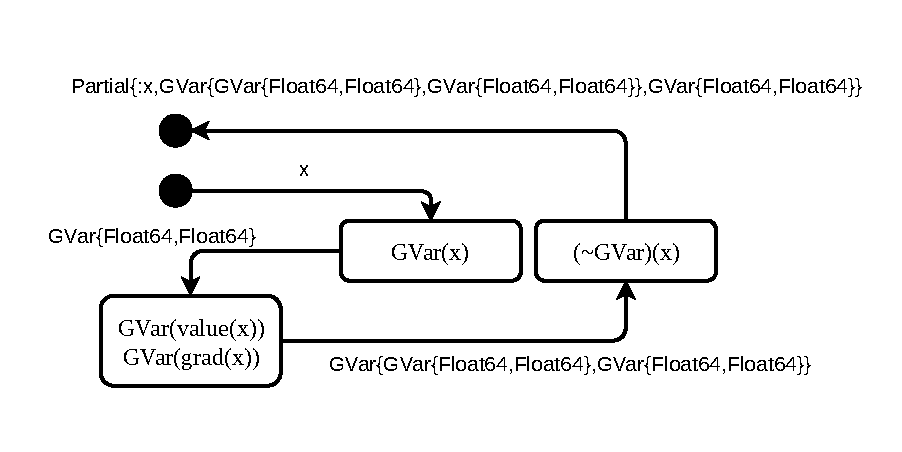
\includegraphics[width=0.9\columnwidth,trim={0 0cm 11cm 0cm},clip]{images/simplehessian.pdf}}
    \caption{Obtaining the second order gradient with the reversive differentiation approach. Colors blue, green, orange and red indicate the four stages, data types and fields used for computation are marked in the same color.}\label{fig:simplehessian}
\end{figure}

Their are four stages in computing Hessian in the naive approach, the first two stages are obtaining gradients, the thrid stage is wrapping each field in \texttt{GVar} with \texttt{GVar} and compute forward function. Then we pick a variable $y$ to compute a row of Hessian by adding $1$ to \texttt{grad($y$)}. At the final stage, the \texttt{$\sim$GVar} operation does not unwrap \texttt{GVar} directly because the gradient field of gradients may be non-zeros. Instead, we use \texttt{Partial\{:FIELD\}($\cdot$)} to savely invert \texttt{GVar} on data type \texttt{GVar\{<:GVar, <:GVar\}}. It take a field without discarding information. In NiLang, \texttt{simple\_hessian} obtains the Hessian matrix in this way by iterating over different $y$s.

The back propagation approach can be more efficient in obtaining higher order gradients.

\begin{minipage}{.44\textwidth}
\begin{lstlisting}
julia> out!, x = 0.0, 1.6
(0.0, 1.6)

julia> @instr iexp''(Loss(out!), x)

julia> collect_hessian()
2×2 Array{Float64,2}:
 0.0  0.0
 0.0  4.95303
\end{lstlisting}
\end{minipage}
\texttt{iexp\textquotesingle\textquotesingle} computes the second order derivative by wrapping the variable into type \texttt{BeijingRing}. This is a special data structure to store Hessians. Whenever an $n$-th variable is created, we push a ring of size $2n-1$ in to a global tape. Whenever an ancilla is deallocated, we pop a ring from the top. The $n$-th ring stores $H_{i\leq n,n}$ and $H_{n,i<n}$. We didn't use the symmetry relation $H_{i,j} = H_{j,i}$ here to simplify the implementation of backward rules described in the right most panel of \Fig{fig:ad}.
The final result can be collected by calling a global function \texttt{collect\_hessian}.

\subsection{QR decomposition}

Not only simple functions, linear algebra functions 

\begin{minipage}{.44\textwidth}
\begin{lstlisting}
@i function iqr(Q, R, A::AbstractMatrix{T}) where T
    @anc anc_norm = zero(T)
    @anc anc_dot = zeros(T, size(A,2))
    @anc ri = zeros(T, size(A,1))
    for col = 1:size(A, 1)
        ri .+= identity.(A[:,col])
        for precol = 1:col-1
            idot(anc_dot[precol], Q[:,precol], ri)
            R[precol,col] += identity(anc_dot[precol])
            for row = 1:size(Q,1)
                ri[row] -= anc_dot[precol] * Q[row, precol]
            end
        end
        inorm2(anc_norm, ri)

        R[col, col] += anc_norm^0.5
        for row = 1:size(Q,1)
            Q[row,col] += ri[row] / R[col, col]
        end

        ~(ri .+= identity.(A[:,col]);
        for precol = 1:col-1
            idot(anc_dot[precol], Q[:,precol], ri)
            for row = 1:size(Q,1)
                ri[row] -= anc_dot[precol] * Q[row, precol]
            end
        end;
        inorm2(anc_norm, ri)
        )
    end
end
\end{lstlisting}
\end{minipage}

where \texttt{idot} and \texttt{inorm2} are implemented as

\begin{minipage}{.44\textwidth}
\begin{lstlisting}
@i function idot(out, v1::AbstractVector{T}, v2)
        where T
    @anc anc1 = zero(T)
    for i = 1:length(v1)
        anc1 += identity(v1[i])
        CONJ(anc1)
        out += v1[i]*v2[i]
        CONJ(anc1)
        anc1 -= identity(v1[i])
    end
end

@i function inorm2(out, vec::AbstractVector{T})
        where T
    @anc anc1 = zero(T)
    for i = 1:length(vec)
        anc1 += identity(vec[i])
        CONJ(anc1)
        out += anc1*vec[i]
        CONJ(anc1)
        anc1 -= identity(vec[i])
    end
end
\end{lstlisting}
\end{minipage}

One can easily check the gradient of this naive implementation of QR decomposition is correct

\begin{minipage}{.44\textwidth}
\begin{lstlisting}
using Test
A = randn(4,4)
q = zero(A)
r = zero(A)

@i function test1(out, q, r, A)
    iqr(q, r, A)
    out += identity(q[1,2])
end

@i function test2(out, q, r, A)
    iqr(q, r, A)
    out += identity(r[1,2])
end

@test check_grad(test1, (Loss(0.0), q, r, A);
        atol=0.05, verbose=true)
@test check_grad(test2, (Loss(0.0), q, r, A);
        atol=0.05, verbose=true)
\end{lstlisting}
\end{minipage}

Here, the \texttt{check\_grad} function is a gradient checker function defined in \texttt{NiLangCore.ADCore}.

\subsection{Unitary Matrices}
Recurrent networks with a unitary parametrized network ease the gradient exploding and vanishing problem~\cite{Arjovsky2015,Wisdom2016,Li2016}.
One of the simplest way to parametrize a unitary matrix is representing a unitary matrix as a product of two-level unitary operations~\cite{Li2016}. A unitary matrix of size $N\times N$ can be parametrized by $k = N(N-1)/2$ two level unitary matrices~\cite{Li2013}. A two-level unitary matrices can be applied in $O(1)$ time. A real unitary matrix can be parametrized compactly by $k$ rotation operations \texttt{ROT(a!, b!, $\theta$)}, where \texttt{$\theta$} is the rotation angle, \texttt{a!} and \texttt{b!} are target registers.

\begin{align}
    {\rm ROT}(a!, b!, \theta)  = \begin{bmatrix}
        \cos(\theta) & - \sin(\theta)\\
        \sin(\theta)  & \cos(\theta)
    \end{bmatrix}
    \begin{bmatrix}
        a!\\
        b!
    \end{bmatrix}
\end{align}


\begin{minipage}{.44\textwidth}
\begin{lstlisting}
@i function umm!(x, θ)
    @anc k = 0
    @anc Nin = size(x, 2)
    @anc Nout = size(x, 1)
    for j=1:Nout
        for i=Nin-1:-1:j
            k += identity(1)
            ROT(x[i], x[i+1], θ[k])
        end
    end

    # uncompute k
    for j=1:Nout
        for i=Nin-1:-1:j
            k -= identity(1)
        end
    end
end
\end{lstlisting}
\end{minipage}

Its backward rule of a \texttt{ROT} instruction is
\begin{align}
    \begin{split}
    \overline{\theta}  &= \sum\frac{\partial R(\theta)}{\partial \theta}\odot(\overline{y}x^T)\\
    &= \Tr\left[\frac{\partial R(\theta)}{\partial \theta}^T\overline{y}x^T\right]\\
    &= \Tr\left[R\left(\frac{\pi}{2}-\theta\right)\overline{y}x^T\right]
    \end{split}
\end{align}

We bind the adjoint function of \texttt{ROT} to its reverse \texttt{IROT},
and define a new function that dispatch to \texttt{GVar} variables

\begin{minipage}{.44\textwidth}
\begin{lstlisting}
@i function IROT(a!::GVar, b!::GVar, θ::GVar)
    IROT(value(a!), value(b!), value(θ))
    NEG(value(θ))
    value(θ) -= identity(π/2)
    ROT(grad(a!), grad(b!), value(θ))
    grad(θ) += value(a!) * grad(a!)
    grad(θ) += value(b!) * grad(b!)
    value(θ) += identity(π/2)
    NEG(value(θ))
    ROT(grad(a!), grad(b!), π/2)
end
\end{lstlisting}
\end{minipage}

\section{Discussion and outlook}\label{sec:discussion}
In this paper, we introduce differential programing on a reversible Turing machine implemented as a Julia eDSL.
It is able to differentiate over any program consisting of instructions and control flows to any order reliablely without sophisticated design of computational graph and intermediate state caching.
Besides automatic differentiation, we introduce a new training strategy learn by consistency that does not rely on gradients.

In the following, we discussed the paractical side of writting reversible programs, and several future directions to go.
Notablely, we introduce the concept of ``arithematic uncomputing'' to reduce the overhead of recursive reversible algorithms.

\subsection{Time Space Tradeoff}\label{sec:timespace}
So far, we have introduced the eDSL. There are many other designs of reversible language and instruction set.
The reversible Turing machine may have either a space overhead propotional to computing time $T$ or a computational overhead that sometimes can be even exponential given limited space.
In the simplest g-segment trade off scheme~\cite{Bennett1989,Levine1990}, it takes $Time(T) = T^{\log _g(4g-2)}$ and $Space(T) = (g-1)S\log_g T$.
This section, we try to convince the reader that the overhead of reversible computing is not as terrible as people thought.

First, one should notice that even in the worst case, the overhead of a reversible program is not more than a traditional machine learning package. In pytorch, a tensor memorize every input of a primitive. The program is apparently reversible since it does not discard any information.
For deep neural networks, people used checkpointing trick to trade time with space~\cite{Chen2016}, which is also a widely used trick in reversible programming~\cite{Perumalla2013}. Reversible programming AD is sometimes more memory efficient. Comparing with logging computational graph, reversible programming has the advantage of supporting inplace functions, which is difficult is both tranditional and source to source AD framework. The example of parametrizing unitary matrice costs zero memory allocation.

Second, some computational overhead of running recursive algorithms with limited space resources can be mitigated by "pseudo uncomputing" without sacrifising reversibility like in the \texttt{iexp} example.

Third, making reversible programming an eDSL rather than a independant language allows flexible choices between reversibility and computational overhead. For example, in order to deallocate the gradient memory in a reversible language one has to uncompute the whole process of obtaining this gradient.
In this eDSL, we can just deallocate the memory irreversibly, i.e. trade energy with time. This underlines the fact that a reversible program is more suited in a program with small granularity. We can quantify it by introducing
\begin{definition}[program granularity]
    The logarithm of the ratio between the execution time of a reversible program and its irreversible counter part.
    \begin{equation}
        \log_2 \frac{Time(T)}{T}
    \end{equation}
\end{definition}

In the lowest granuality, instruction design, we need ancilla bits. Defining primitive functions like \texttt{iexp} requires uncomputing ancillas. Deallocating the gradient further increase the granularity by $\sim 1$. After the training, the inverse training of whole programs should be done to deallocate all the memory used for training. As a result, the program complexity increase exponentially as the granuality increase.
The granularity can be decreased by flattening the functions, since the uncomputing of ancillas can be executed at any level of granularity.

One should notice the memory advantage of reversible programming to machine learning does comes from reversibility itself, but from a better data tracking strategy inspired from invertible programming.
Normally, a reversible program is not as memory efficient as its irreversible couterpart due to the additional requirement of no information loss. A naive approach that keeping track of all informations will cost an additional space $O(T)$, where $T$ stands for the excution time in a irreversible TM, the longer the program runs, the larger the memory usage is. This is exactly the approach to keeping reversibility in most machine learning packages in the market.
The point it, an reversible Turing Machine is able to trade space with time.
In some cases, it may cause polynomial overhead than its irreversible counterpart.

\subsection{Instructions and Hardwares}\label{sec:instruction}
%Todays CPU are starving, that is, the memory access is the performance bottleneck in many applications rather than the arithmetic operations.
%There is a natural granularity for operations with memory access or not.
So far, our eDSL is not really compiled to instructions, instead it runs on a irreversible host Julia.
In the future, it can be compiled to low level instructions and is executable on a reversible devices.
For example, the control flow defined in this NiLang can be compiled to reversible instructions like conditioned \texttt{goto} statement.
It is designed in such a way that the target instruction is a \texttt{comefrom} statement which specifies the postcondition. ~\cite{Vieri1999}

Arithmetic instructions should be redesigned to support better reversible programs.
The major obstacle to exact reversibility programming is current floating point adders used in our computing devices are not exactly reversible.
There are proposals of reversible floating point adders~\cite{Nachtigal2011,Nguyen2013} that introduces garbage bits to ensure reversibility.
In other words, to represent a 64 bit floating point number requires more than 64 bits in storage. Reversible multiplier is also possible in similar approach.~\cite{Nachtigal2010} With these infrastructure, a reversibile program can be executed without suffereing from the irreversibility from rounding error.
In machine learning field, people using information buffer in multiplication operations~\cite{Maclaurin2015} in an approach to enforce invertibility in a memory efficient way.

Reversible programming is not nessesarily related to reversible hardwares, reversible programs is a subset of irreversible programs hence can be simulated efficiently with CMOS technologies~\cite{Vieri1999}. However, only using reversible hardwares~\cite{} can break the energy efficiency barrier by Landauer principle.
Reversible hardwares are not nessesarily related to reversible gates such as Toffoli gate and Fredkin gate.
Devices with the ability of recovering signal energy is able able to save energy, which is known as generalized reversible computing.~\cite{Frank2005,Frank2017b}
In the following, we comment briefly on a special type of reversible device Quantum computer.

\subsection{Quantum Computers}\label{sec:qc}
One of the fundamental difficulty of building a quantum computer is, unlike a classical state, an unknown quantum state can not be copied.
Quantum random access memory~\cite{Giovannetti2008} is very hard to design and implement, it is known to have many caveats~\cite{Aaronson2015}.
A quantum state in a environment will decoherence and can not be recovered, this underlines the simulation nature of quantum devices.
%In the era of noisy intermediate sized quantum devices, more and more people are switching to classical-quantum hybrid devices, where a quantum device plays the role of a programmable simulator.
Reversible computing does not enjoy the quantum advantage from entanglement, nor the quantum disadvantages from non-cloning and decoherence.
Only the limitation of reversibility is retained, reversibility comes from the fact that micro scopic processes are all unitary.
In microscopic world, irreversibility is rare, it can come from the interaction with classical devices, like environment induces decaying, qubit state resetting, measurements and classical feedbacks to quantum devices. These are typically harder to implement on a quantum device.

Given the fundamental limitations of quantum decoherence and non-cloning and the microscopic reversible nature.
It is reasonable to have a reversible computing device to bridge the gap between classical and universal quantum computing.
By introducing entanglement little by little, we can accelerate some basic components like a reversible adder.
The quantum fourier transformation provides a shortcut to the adder bt introducing only one additional gate, the CPHASE gate even though it is a classical in classical out algorithm.~\cite{} Interestingly, by introducing rotation gates $Ry(\theta)$ and $Rz(\theta)$ in the reversible programming, we make NiLang a path integral based universal quantum simulator as shown in \App{app:quantum}. The compiling theory developed for reversible programming will have profounding effect to quantum computers.

\subsection{Outlook}\label{sec:outlook}
So far NiLang is not full ready for productivility. It can be improved from multiple perspectives, compiling support to merge the uncomputing can decrease granularity and hence reduce overhead. Additional instructions like stack operations and logical operations are under consideration. It is also interesting to see how it can be combined with a high performance quantum simulator like \texttt{Yao}. It is able to provide control flow to \texttt{Yao}'s QBIR. By porting a quantum simulator. it is interesting to see how quantum simulator can improve the instruction design. Notice a quantum fourier transformation (QFT) based quantum adder and multiplier is sometimes more efficient than a classical adder~\cite{Haener2018} \blue{Is this true?}.
Reversible programming is known to have the advantage in parallel computing~\cite{Jefferson1985} and debugging~\cite{Boothe2000}, it is interesting to see how it combines with other parts of Julia packages like CUDAnative~\cite{Besard2018} and Debugger, it would be interesting to see our eDSL running on a GPU with little synchronization overhead~\blue{Is this even possible?} and using an interative debugging with bidirectional move.
This could be used to reduce the momory cost in normalizing flow, time reversible integrator, recurrent neural network and residual neural network.

\section{acknowledgments}
Jin-Guo Liu thank Lei Wang for motivating the project with possible applications reversible integrator, normalizing flow and neural ODE.
Xiu-Zhe Luo for discussion on the implementation details of source to source automatic differetiation,
Shuo-Hui Li for helpful discussion on differential geometry.
Damian Steiger for telling me the \texttt{comefrom} joke.
Tong Liu and An-Qi Chen for helpful discussion on quantum adders and multipliers.
The authors are supported by the National Natural Science Foundation of China under the Grant No.~11774398, the Strategic Priority Research Program of Chinese Academy of Sciences Grant No.~XDB28000000 and the research funding from Huawei Technologies under the Grant No.~YBN2018095185.

\bibliographystyle{apsrev4-1}
\bibliography{invc}

\pagebreak
\appendix

\section{NiLang Grammar}\label{app:grammar}

Terminologies
\begin{itemize}
    \item $ident$, symbols
    \item $num$, numbers
    \item $\epsilon$, empty statement
    \item $JuliaExpr$, native julia expression
    \item $[$ $]$,  zero or one repetitions.
\end{itemize}

\begin{minipage}{0.3\textwidth}
    \small
\begin{bnf*}
    \bnfprod{Stmts}{\bnfsp \bnfes}\\
    \bnfmore{\bnfor \bnfpn{Stmt}}\\
    \bnfmore{\bnfor \bnfpn{Stmts} \bnfsp \bnfpn{Stmt}}\\
    \bnfprod{Stmt}{\bnfpn{BlockStmt}}\\
    \bnfmore{\bnfor \bnfpn{IfStmt}}\\
    \bnfmore{\bnfor \bnfpn{WhileStmt}}\\
    \bnfmore{\bnfor \bnfpn{ForStmt}}\\
    \bnfmore{\bnfor \bnfpn{InstrStmt}}\\
    \bnfmore{\bnfor \bnfpn{RevStmt}}\\
    \bnfmore{\bnfor \bnfpn{@anc} \bnfsp \bnfpn{Stmt}}\\
    \bnfmore{\bnfor \bnfpn{@routine} \bnfsp \bnfpn{Stmt}}\\
    \bnfmore{\bnfor \bnfpn{@safe} \bnfsp \bnftd{$JuliaExpr$}}\\
    \bnfmore{\bnfor \bnfpn{CallStmt}}\\
    \bnfprod{BlockStmt}{\bnftd{begin} \bnfsp \bnfpn{Stmts} \bnfsp \bnftd{end}}\\
    \bnfprod{RevCond}{\bnftd{(} \bnfsp \bnftd{$JuliaExpr$} \bnfsp \bnftd{,} \bnfsp \bnftd{$JuliaExpr$} \bnfsp \bnftd{)}}\\
    \bnfprod{IfStmt}{\bnftd{if} \bnfsp \bnfpn{RevCond} \bnfsp \bnfpn{Stmts} \bnfsp \bnfts{[} \bnftd{else} \bnfsp \bnfpn{Stmts}\bnfts{]} \bnfsp \bnftd{end}}\\
    \bnfprod{WhileStmt}{\bnftd{while} \bnfsp \bnfpn{RevCond} \bnfsp \bnfpn{Stmts} \bnfsp \bnftd{end}}\\
    \bnfprod{Range}{\bnftd{$JuliaExpr$} \bnfsp \bnftd{:} \bnfsp \bnftd{$JuliaExpr$} \bnfsp \bnfts{[} \bnftd{:} \bnfsp \bnftd{$JuliaExpr$}\bnfts{]}}\\
    \bnfprod{ForStmt}{\bnftd{for} \bnfsp \bnftd{ident} \bnfsp \bnftd{=} \bnfsp \bnfpn{Range} \bnfsp \bnfpn{Stmts} \bnfsp \bnftd{end}}\\
    \bnfprod{CallStmt}{\bnftd{$JuliaExpr$} \bnfsp \bnftd{(} \bnfsp \bnfts{[} \bnfpn{DataViews}\bnfts{]} \bnfsp \bnftd{)}}\\
    \bnfprod{Constant}{\bnftd{num} \bnfor \bnftd{$\pi$}}\\
    \bnfprod{InstrBinOp}{\bnftd{+=} \bnfor \bnftd{-=} \bnfor \bnftd{$\veebar$=}}\\
    \bnfprod{InstrTrailer}{\bnfts{[} \bnftd{.}\bnfts{]} \bnfsp \bnftd{(} \bnfsp \bnfts{[} \bnfpn{DataViews}\bnfts{]} \bnfsp \bnftd{)}}\\
    \bnfprod{InstrStmt}{\bnfpn{DataView} \bnfsp \bnfpn{InstrBinOp} \bnfsp \bnftd{ident} \bnfsp \bnfts{[} \bnfpn{InstrTrailer}\bnfts{]}}\\
    \bnfprod{RevStmt}{\bnftd{$\sim$} \bnfsp \bnfpn{Stmt}}\\
    \bnfprod{@routine}{\bnftd{@routine} \bnfsp \bnftd{ident} \bnfsp \bnfpn{Stmt}}\\
    \bnfprod{AncArg}{\bnftd{ident} \bnfsp \bnftd{=} \bnfsp \bnftd{$JuliaExpr$}}\\
    \bnfprod{@anc}{\bnftd{@anc} \bnfsp \bnfpn{AncArg}}\\
    \bnfmore{\bnfor \bnftd{@deanc} \bnfsp \bnfpn{AncArg}}\\
    \bnfprod{@safe}{\bnftd{@safe} \bnfsp \bnftd{$JuliaExpr$}}\\
    \bnfprod{DataViews}{\bnfsp \bnfes}\\
    \bnfmore{\bnfor \bnfpn{DataView}}\\
    \bnfmore{\bnfor \bnfpn{DataViews} \bnfsp \bnftd{,} \bnfsp \bnfpn{DataView}}\\
    \bnfprod{DataView}{\bnfpn{DataView} \bnfsp \bnftd{[} \bnfsp \bnftd{$JuliaExpr$} \bnfsp \bnftd{]}}\\
    \bnfmore{\bnfor \bnfpn{DataView} \bnfsp \bnftd{.} \bnfsp \bnftd{ident}}\\
    \bnfmore{\bnfor \bnftd{$JuliaExpr$} \bnfsp \bnftd{(} \bnfsp \bnfpn{DataView} \bnfsp \bnftd{)}}\\
    \bnfmore{\bnfor \bnfpn{Constant}}\\
    \bnfmore{\bnfor \bnftd{ident}}\\
\end{bnf*}

\end{minipage}

One can use \texttt{@i function $\<Stmts\>$ end} to define a function and its inverse. All $JuliaExpr$ is should be pure, otherwise the reversibility is not gurantted.

Dataview is a bijective mapping of an object or a field (or item) of an object.
When modifying the dataview of an object, it changes the object directly with the \texttt{chfield} method.

\section{Instruction Table}\label{app:instr}

The translation of instructions to Julia functions
\begin{table}[h!]\centering
\begin{minipage}{\columnwidth}
\ra{1.3}
    \scalebox{1.0}{
        \begin{tabularx}{\textwidth}{X X X}\toprule
            \textbf{instruction} & \textbf{translated} & \textbf{type}\\
            \hline
            $y \pluseq f(args...)$ & $\oplus(f)(args...)$ & \texttt{PlusEq}\\
            $y \minuseq f(args...)$ & $\ominus(f)(args...)$ & \texttt{MinusEq}\\
            $y \mathrel{\veebar}= f(args...)$ & $\odot(f)(args...)$ & \texttt{XorEq}\\
            \bottomrule
        \end{tabularx}
    }
    \caption{Instructions and their interpretation in NiLang.}\label{tbl:interp}
\end{minipage}
\end{table}


The list of instructions implemented in NiLang
\begin{table}[h!]\centering
\begin{minipage}{\columnwidth}
\ra{1.3}
    \scalebox{1.0}{
        \begin{tabularx}{\textwidth}{X X}\toprule
            \textbf{instruction} & \textbf{output}\\
            \hline
            ${\rm SWAP}(a, b)$ & $b, a$\\
            ${\rm ROT}(a, b, \theta)$ & $a \cos\theta - b\sin\theta, b \cos\theta + a\sin\theta, \theta$\\
            ${\rm IROT}(a, b, \theta)$ & $a \cos\theta + b\sin\theta, b \cos\theta - a\sin\theta, \theta$\\
            $y \pluseq a^\wedge b$ & $y+a^b, a, b$\\
            $y \pluseq \exp(x)$ & $y+e^x, x$\\
            $y \pluseq \log(x)$ & $y+\log x, x$\\
            $y \pluseq \sin(x)$ & $y+\sin x, x$\\
            $y \pluseq \cos(x)$ & $y+\cos x, x$\\
            $y \pluseq {\rm abs}(x)$ & $y+ |x|, x$\\
            ${\rm NEG}(y)$ & $-y$\\
            ${\rm CONJ}(y)$ & $y'$\\
            \bottomrule
        \end{tabularx}
    }
    \caption{A collection of reversible instructions.}\label{tbl:revinstructions}
\end{minipage}
\end{table}


\end{document}
